\documentclass[11pt]{article}

% --------------------------------------------------
% Packages
% --------------------------------------------------
\usepackage[margin=1in]{geometry}
\usepackage{amsmath, amssymb, amsthm}
\usepackage{mathtools}
\usepackage{graphicx}
\usepackage{float}
\usepackage{enumitem}
\usepackage{hyperref}
\usepackage{xcolor}
\usepackage{tikz}
\usetikzlibrary{arrows.meta, positioning, calc, shapes}

% Pseudocode and algorithms
\usepackage{algorithm}
\usepackage{algpseudocode}

% Better fonts (optional)
\usepackage{lmodern}

% --------------------------------------------------
% Hyperref setup
% --------------------------------------------------
\hypersetup{
    colorlinks=true,
    linkcolor=blue,
    citecolor=blue,
    urlcolor=blue
}

% --------------------------------------------------
% Theorem-like environments
% --------------------------------------------------
\theoremstyle{definition}
\newtheorem{definition}{Definition}[section]
\newtheorem{theorem}{Theorem}[section]
\newtheorem{claim}{Claim}[section]
\newtheorem{remark}{Remark}[section]
\newtheorem{recall}{Recall}[section]

% --------------------------------------------------
% Custom commands
% --------------------------------------------------
\newcommand{\Gen}{\mathsf{Gen}}
\newcommand{\Enc}{\mathsf{Enc}}
\newcommand{\Dec}{\mathsf{Dec}}
\newcommand{\Sig}{\mathsf{Sig}}
\newcommand{\Ver}{\mathsf{Ver}}
\newcommand{\negl}{\mathsf{negl}}

% --------------------------------------------------
% Document
% --------------------------------------------------
\begin{document}

\title{Public Key Crypto notes - 09}
\author{By contributors}
\date{April 13. 2026}
\maketitle

% --------------------------------------------------
\section{PoK protocols we learnt about}
% --------------------------------------------------

\begin{recall}[Proof-of-knowledge protocols]\leavevmode
	\begin{enumerate}
		\item $\text{PoK}[x:g^x = h](m) \leftarrow$ Schnorr signature
		\item $\text{PoK}[x: g^{a^x} = y](m)$, $g, a, y$ are public
	\end{enumerate}
\end{recall}

\section{New PoK protocol - PoK RootLog}

\begin{itemize}
	\item Public parameters: $g, e, y$
	\item Goal: Prover knows $x$ such that: $y = g^{(x^e)}$, where $ord(g) = N$ is an RSA modulus.
	\item Two parties: $Prover(x)$ and $Verifier(g, N, e, y)$ who know all public parameters.
	\begin{enumerate}
		\item The Prover chooses $k \in_R {1, \dots, 2^\lambda}$, $t = g^{(k^e)}$, where $\lambda$ is a security parameter. The commitment $t$ is sent to the Verifier.
		\item The Verifier chooses $r \in_R \{0, 1\}$ and sends it to the Prover.
		\item The Prover checks: $s = \begin{cases}
			k, \text{ if } r = 0 \\
			\frac{k}{x}, \text{ if } r = 1
		\end{cases}$, where $x$ is the to-be-proved value of the Prover, and sends $s$ to the Verifier.
		\item The Verifier checks: $t \stackrel{?}{=} \begin{cases}
			g^{(s^e)}, \text{ if } r = 0 \\
			y^{(s^e)}, \text{ if } r = 1
		\end{cases}$
	\end{enumerate}
	\item Correctness: $r = 0 \checkmark \\
	r = 1: y^{(s^e)} = y^{(\frac{k}{x}^e)} = g^{(x^e) \cdot (\frac{k}{x})^e} = g^{(k^e)} = t$
	\item Success probability: $\frac{1}{2}$, so to achieve negligible probability that the Prover succeeds with proving an incorrect value, we need to iterate the protocol several times.
\end{itemize}

\subsection{Non-interactive version}

\begin{itemize}
	\item For $i = 1, \dots$: $t_i = g^{(k_i)^e}$ with random $k_i$, $r = H(m || y || g || e || t_1 || t_2 || \dots)$
	\item $s_i = \begin{cases}
		k_i, \text{ if } r_i = 0 \\
		\frac{k_i}{x}, \text{ if } r_i = 1
	\end{cases}$, where $r = r_1 || r_2 || r_3 || \dots$.
	\item PoK $x: y = g^{(x^e)}(m) = (r, s_1, s_2, \dots)$
\end{itemize}

\section{Group signatures continued}

\begin{tikzpicture}[
	>=Stealth,
	node distance=2cm,
	signer/.style={circle, draw, minimum size=8mm},
	manager/.style={rectangle, draw, rounded corners, minimum width=2.5cm, minimum height=1cm},
	output/.style={rectangle, draw, minimum width=3cm, minimum height=1cm},
	group/.style={draw, ellipse, minimum width=6cm, minimum height=4cm}
	]
	
	% Group G
	\node[group] (G) {};
	\node at (G.north) [yshift=4mm] {$G$};
	
	% Signers
	\node[signer] (S1) at (-1.5,0.5) {$S_1$};
	\node[signer] (S2) at (-0.5,-0.7) {$S_2$};
	\node[signer] (S3) at (-2,-0.8) {$S_3$};
	\node[signer] (Si) at (1.5,0.3) {$S_i$};
	
	\node at (0,-1.6) {$\ldots$};
	
	% Output (message, signature)
	\node[output, right=3cm of Si] (out) {$(m,\sigma)$};
	
	% Arrow from signer to output
	\draw[->] (Si) -- node[above] {sign} (out);
	
	% Manager
	\node[manager, above=2cm of G] (M) {Manager $M$};
	
	% Manager actions
	\draw[->, dashed] (M) -- node[left] {add} (G);
	\draw[->, dashed] (M) -- node[right] {remove} (G);
	
\end{tikzpicture}

\begin{itemize}
	\item Setup:
	\begin{itemize}
		\item $M$ computes:
		\begin{itemize}
			\item $(N, c), (N, d)$ RSA keys
			\item A prime $p$ and $g \in \mathbb{Z}_p^*$ such that $ord_p(g) = N$
			\item $a \in \mathbb{Z}_N^*$ with large order
			\item Public key: $(p, g, N, e, a)$, secret key: $d$
		\end{itemize}
	\end{itemize}
	\item Join:
	\begin{itemize}
		\item $x_i$ random
		\item $y_i = a^{x_i} \pmod{N}$
		\item $z_i = g^{y_i}$, where $z_i$ is called the membership key
		\item $(y_i, z_i)$ is sent to $M$ with PoK$[\alpha: a^\alpha = y_i]$
		\item $M$ returns $v_i = (y_i + 1)^d$
		\item $M$ stores $y_i$ in $\mathcal{Y}$
	\end{itemize}
	\item Sign:
	\begin{itemize}
		\item $S_i$ computes:
		\begin{itemize}
			\item $r \in_R \mathbb{Z}_N$
			\item $\tilde{g} = g^r$ (blinded $g$)
			\item $\tilde{z} = \tilde{g}^{y_i}$
			\item $V_1 = \text{PoK}[\alpha: \tilde{z} = \tilde{g}^{a^\alpha}](m)$
			\item $V_2 = \text{PoK}[\beta \cdot \tilde{z} \cdot \tilde{g} = \tilde{g}^{\beta^e}](m)$
			\item Signature = $\tilde{g}, \tilde{z}, V_1, V_2$
		\end{itemize}
	\end{itemize}
	\item Open:
	\begin{itemize}
		\item Given $(\tilde{g}, \tilde{z}, V_1, V_2)$
		\item Let $\mathcal{Y}$ be the list of $y_i$ values
		\item Then, check: $\tilde{g}^{y_i} \stackrel{?}{=} \tilde{z}$ for all $y_i \in \mathcal{Y}$
	\end{itemize}
	\item Correctness:
	\begin{itemize}
		\item By $V_1,$ $\tilde{g} \cdot \tilde{z}$ has the form $\tilde{g}^{y_i + 1}$
		\item By $V_2$, $S_i$ knows $(y_i + 1)^d = V_i$
	\end{itemize}
\end{itemize}

\section{Elliptic Curve Cryptography (ECC)}

\subsection{Motivation}

\begin{itemize}
	\item Diffie-Hellman key exchange
	\item Two users, $A, B$, they have secret keys $a, b$, and public keys $g^a, g^b \pmod{p}$
	\item It is secure if the discrete log problem is hard
	\item Having index calculus $p$ must have bit size 3000-4000 (almost one megabyte)
	\item Using elliptic curves, we can have sufficiently secure key sizes of 200-500 bits
\end{itemize}

\begin{definition}[Elliptic curve]
	An elliptic curve $E$ over $\mathbb{R}$ is a set of points:
	$$
	E = E_{A, B} = \{(x, y): y^2 = x^3 + Ax + B\} \cup \{\infty\}
	$$
	with $A, B \in \mathbb{R}$, such that $4A^3 + 27B^2 \ne 0$.
\end{definition}

\begin{figure}[H]
	\centering
	\begin{tikzpicture}[scale=1.0]
		% Axes
		\draw[->] (-3,0) -- (4,0) node[right] {$x$};
		\draw[->] (0,-3) -- (0,3) node[above] {$y$};
		
		% Shift amount
		\def\xzero{1.0}
		
		% Curve: y^2 = (x-x0)^3, parametrized by (x0+t^2, t^3)
		\draw[thick, blue, domain=-1.4:1.4, samples=200, smooth]
		plot ({\xzero + \x*\x}, {\x*\x*\x});
		
		% Singular point
		\filldraw[red] (\xzero,0) circle (2pt) node[below] {$x_0$};
		
		\node[blue] at (2.5,2.1) {$y^2=(x-x_0)^3$};
	\end{tikzpicture}
	\caption{Singular cubic with a triple root translated to $x=x_0$.}
\end{figure}

Case 2: Normal elliptic curve

\begin{figure}[H]
	\centering
	\begin{tikzpicture}[scale=1.0]
		% Axes
		\draw[->] (-2.4,0) -- (2.8,0) node[right] {$x$};
		\draw[->] (0,-2.8) -- (0,2.8) node[above] {$y$};
		
		% Elliptic curve y^2 = x^3 - x + 1
		% Use a slightly safer left endpoint to avoid sqrt of a negative number
		\draw[thick, blue, domain=-1.324:2.0, samples=300, smooth]
		plot (\x, {sqrt(\x*\x*\x - \x + 1)});
		\draw[thick, blue, domain=-1.324:2.0, samples=300, smooth]
		plot (\x, {-sqrt(\x*\x*\x - \x + 1)});
		
		% Label
		\node[blue] at (1.45,2.15) {$y^2 = x^3 - x + 1$};
	\end{tikzpicture}
	\caption{A normal (nonsingular) elliptic curve over $\mathbb{R}$.}
\end{figure}

\begin{remark}
	$E$ is symmetric to the $x$-axis: $(x, y) \in E$ if and only if $(x, -y) \in E$.
\end{remark}

$f(x) = x^3 + Ax + B$ is cubic

Case 1: 3 different zeros

Case 2: 1 zero

\begin{itemize}
	\item $D(A, B) = 4A^3 + 27B^2$ is the discriminant of the cubic $f(x) = x^3 + Ax +b$
	\item $f(x)$ has multiple zeros if $D(A, B) = 0$
	\item Case 1: $D(A, B) = 0, f(x) = (x-x_0)^3$
	\item Case 2: $D(A, B) = 0, f(x) = (x-x_0)^2 (x-x_1)$
\end{itemize}

\begin{figure}[H]
	\centering
	\begin{tikzpicture}[scale=1.0]
		% Axes
		\draw[->] (-3,0) -- (3,0) node[right] {$x$};
		\draw[->] (0,-3) -- (0,3) node[above] {$y$};
		
		% Nodal cubic: y^2 = x^2(x+1)
		% Parametrize upper/lower branches as y = ±sqrt(x^2(x+1)), for x >= -1
		\draw[thick, blue, domain=-1:2.2, samples=200, smooth]
		plot (\x, {sqrt((\x*\x)*(\x+1))});
		\draw[thick, blue, domain=-1:2.2, samples=200, smooth]
		plot (\x, {-sqrt((\x*\x)*(\x+1))});
		
		% Singular point
		\filldraw[red] (0,0) circle (2pt) node[below right] {node};
		
		% Labels
		\node[blue] at (1.4,2.2) {$y^2=x^2(x+1)$};
	\end{tikzpicture}
	\caption{Singular cubic with a double root: a node.}
\end{figure}

\subsection{Addition low of elliptic curves}

\begin{itemize}
	\item Let $P, Q \in E$, we define $P \oplus Q \in E$ (where $\oplus$ is the coordinate-wise addition) by the tangent-and-core method
	\item If $P=Q \rightarrow P \oplus Q = 2P$
	\item Point at infinity: basically the intersection of all vertical lines in the space. It is used when two points have the same $y$ coordinate. The line between these two points reaches the point of infinity. In this case: $P \oplus Q = \infty, P \oplus \infty = P$
\end{itemize}

\begin{figure}[H]
	\centering
	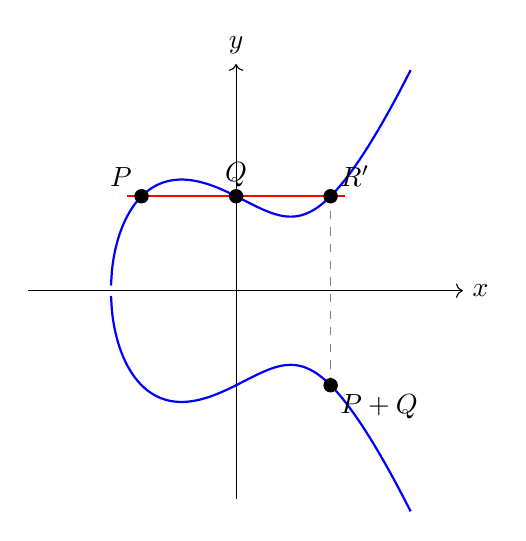
\begin{tikzpicture}[scale=1.2]
		% Axes
		\draw[->] (-2.2,0) -- (2.4,0) node[right] {$x$};
		\draw[->] (0,-2.2) -- (0,2.4) node[above] {$y$};
		
		% Elliptic curve y^2 = x^3 - x + 1
		\draw[thick, blue, domain=-1.324:1.85, samples=300, smooth]
		plot (\x, {sqrt(\x*\x*\x - \x + 1)});
		\draw[thick, blue, domain=-1.324:1.85, samples=300, smooth]
		plot (\x, {-sqrt(\x*\x*\x - \x + 1)});
		
		% Exact points on the curve
		\coordinate (P) at (-1,1);
		\coordinate (Q) at (0,1);
		\coordinate (Rthird) at (1,1);   % third intersection of secant with curve
		\coordinate (Sum) at (1,-1);     % P+Q = reflection of Rthird
		
		% Secant line through P and Q: y = 1
		\draw[red, thick] (-1.15,1) -- (1.15,1);
		
		% Reflection line
		\draw[dashed, gray] (1,-1) -- (1,1);
		
		% Points
		\filldraw[black] (P) circle (2pt) node[above left] {$P$};
		\filldraw[black] (Q) circle (2pt) node[above] {$Q$};
		\filldraw[black] (Rthird) circle (2pt) node[above right] {$R'$};
		\filldraw[black] (Sum) circle (2pt) node[below right] {$P+Q$};
		
		% Optional note
		\node[red] at (0.45,1.18) {};
	\end{tikzpicture}
	\caption{Geometric addition on the elliptic curve $y^2=x^3-x+1$: the line through $P$ and $Q$ meets the curve again at $R'$, and $P+Q$ is the reflection of $R'$ across the $x$-axis.}
\end{figure}

\begin{figure}[H]
	\centering
	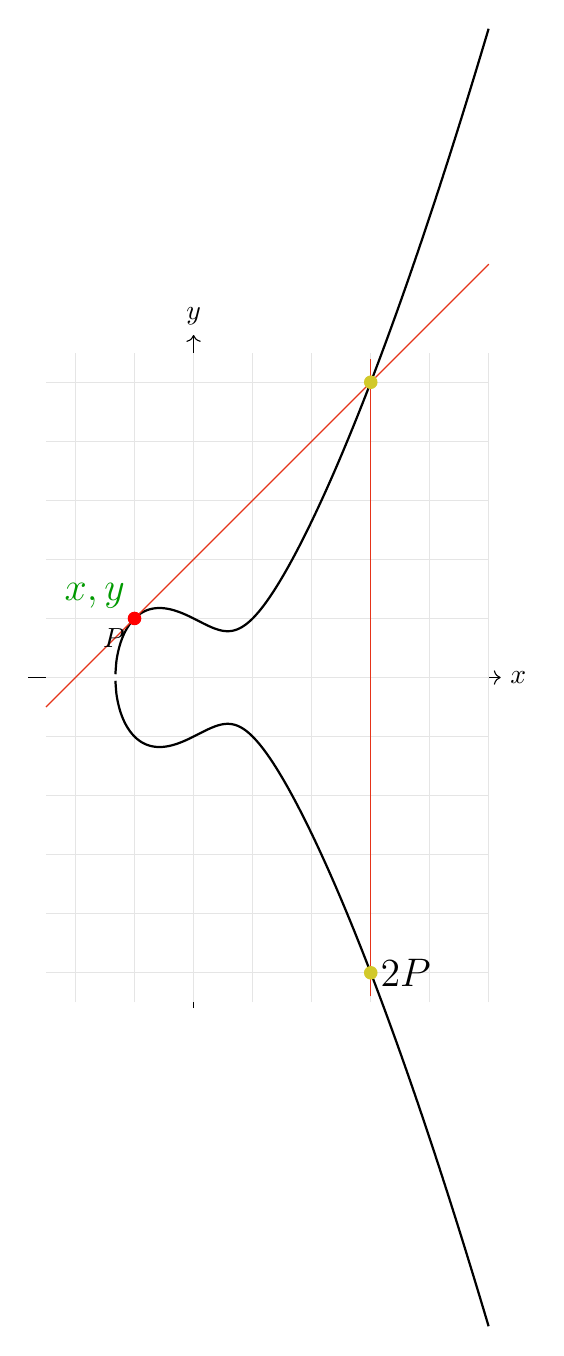
\begin{tikzpicture}[scale=0.75]
		% Axes
		\draw[->] (-2.8,0) -- (5.2,0) node[right] {$x$};
		\draw[->] (0,-5.6) -- (0,5.8) node[above] {$y$};
		
		% Light grid (to resemble the sample)
		\draw[gray!20, step=1] (-2.5,-5.5) grid (5,5.5);
		
		% Elliptic curve: y^2 = x^3 - x + 1
		\draw[thick, black, domain=-1.324:5, samples=400, smooth]
		plot (\x, {sqrt(\x*\x*\x - \x + 1)});
		\draw[thick, black, domain=-1.324:5, samples=400, smooth]
		plot (\x, {-sqrt(\x*\x*\x - \x + 1)});
		
		% Exact points
		\coordinate (P) at (-1,1);
		\coordinate (R) at (3,5);
		\coordinate (D) at (3,-5);
		
		% Tangent line at P: y = x + 2
		\draw[red!60!brown, thin] (-2.5,-0.5) -- (5,7);
		
		% Vertical reflection line through x=3
		\draw[red!60!brown, thin] (3,-5.4) -- (3,5.4);
		
		% Points
		\filldraw[red] (P) circle (3pt);
		\filldraw[yellow!80!black] (R) circle (3pt);
		\filldraw[yellow!80!black] (D) circle (3pt);
		
		% Labels
		\node[below left] at (P) {$P$};
		\node[above left] at (P) {\color{green!60!black}\Large $x,y$};
		
		\node[right] at (D) {\Large $2P$};
	\end{tikzpicture}
	\caption{Point doubling on the elliptic curve $y^2=x^3-x+1$: the tangent at $P=(-1,1)$ meets the curve again at $R=(3,5)$, and $2P=(3,-5)$ is the reflection of $R$ across the $x$-axis.}
\end{figure}

\end{document}